\section{英國人留下來的制度為何九七後就行不通?}

因為特區政府所處的社會、經濟和政治環境已不一樣。表面上,九七前的港英政府同樣欠缺民意授權,受針對的卻是九七後的特區政府,好像是民意對特區政府特別嚴苛似的。然而即使是同一套制度,在不同的時空可帶來完全不同的社會反應。再者,特區政府對同一套制度的具體應用,也和九七前有明顯差別。

其實港英政府也有出現過認授危機,六七暴動就是一例。六七暴動前香港有各種明顯的社會不公,加上貪污橫行警察濫權,為挑戰政權合法性製造了客觀條件。港英政府在七十年代成立廉政公署,又建立各式各樣的社會保障制度,就是對認授危機的回應。到了香港進入九七前的過渡期,高速經濟發展帶來了表現認授,加上社會更關注九七後港人治港的實施,也緩解了港英政府欠缺民意授權的問題。

來到特區政府,先是連續七年的經濟蕭條打破了原來的表現認授,製造了社會對政府能力的嚴重質疑。而九七後港人治港承諾一一落空,政治改革前路越見渺茫,也加劇了政府的認授危機。再者,過去港英政府各種疏解認授危機的手段在特區時代也紛紛變味,問題就被進一步擴大。

港英政府有一個常用的疏解認授危機手段,學界稱之為「行政吸納政治」。香港政府的運作除了受立法會的監管外,尚有數以百計大大小小的委員會協助決策或提供意見。舉個例,要改變土地發展的用途,要先經過城市規劃委員會的審批。若對環境影響評估的結果不滿,又可以找環境影響評估上訴委員會小組。這些委員會的存在要追溯英治的歷史,當時港英政府明白到任何的公共政策都有機會引起社會不滿,而港督本身既非民選所以認授始終有限,與其讓不同利益在政府以外爭吵,不如將它們都納入為管治制度的一部分,一方面讓其代表人物感到被政府尊重,也減低對政府帶來的壓力。例如一些比較有名望的專業人士,可委派他們成為該界別的諮詢委員,讓他們預早為政策制訂提供意見,到政策推出時他們也會幫忙推銷,借助他們的聲望讓業界較易信服。

這些手段要行得通,當權者首要意識到自己的管治地位並非必然,並要有一定的智慧和胸襟,有技巧地平衡不同立場和利益。然而自特區成立以來,這個港英政府的管治法寶在特區政府的手中明顯走樣。各項任命和前文提及行政會議和問責高官的情況一樣,變成了排除異己或回報忠誠的手段。以青年事務委員會為例,本來是六七暴動後成立,原意是讓政府能在官僚體系外更直接地聽到年輕人的聲音,以求盡早回應年輕人的訴求,以免社會動盪重現。現在的青年事務委員會卻被輿論譏為「富二代委員會」,不少委員都是城中富豪的後裔,委員會成為他們刷履歷的地方。現任主席劉鳴煒就是富商劉鑾雄的兒子,曾在談及年輕人置業困難時建議他們應減少去日本旅行多作儲蓄,又向記者大談自己十歲時曾收父母十萬元現金作生日禮物,被廣泛批評為不切實際和不能理解年輕人的真正需要。

另一個相類似而同樣在特區年代變味的制度,就是授勳及嘉獎制度。港英時代在香港有傑出貢獻者,可獲大英帝國勳章,如官佐勳章(OBE)和員佐勳章(MBE)等。其中得到騎士爵位者,可終生冠上爵士或女爵士頭銜(俗稱「阿Sir」)。這些榮耀當然也是政府攏絡人手的手段之一,但條件時過去的授勳者都是德高望重,這樣未來的授勳者才會感到與有榮焉。來到特區時代,同樣的制度卻引起很多爭議。例如香港工會聯合會的前領導人楊光雖然在六七暴動期間擔任鬥委會主任,卻在二零零一年獲得特區最高榮譽的大紫荊勳章,引起公眾嘩然。即使是較不敏感的人物也一樣引起爭論,如藝人安德尊因為服務老人而兩次獲得特區榮譽,反而曾任香港樂施會總幹事而且一直推動盲人平權的莊陳有,則至今從來未獲特區嘉獎。有評論就認為這可能和安德尊願意公開支持建制陣營,而莊陳有則和民主陣營友好有關。當嘉獎變得親疏有別,也就失去了原來提高管治認授的功能。

當任人為親而非用人唯賢的問題蔓延至一些法定組織時,其決策就不免會招來政治蓋過專業的質疑,公眾會認為他們的決定並非出於客觀判斷,而只是為了替行政長官的政治立場護航。例如梁振英在當選特首之後,便在香港大學的校務委員會當中安插多位與他關係友好的人士出任委員。到了曾多次公開批評梁振英的知名法律學者陳文敏被推薦成為港大副校長時,遴選工作便出現眾多轉折,最後任命被校務委員會否決。事件當中與梁振英友好的委員的表現受到廣泛質疑,反對任命的理據錯謬百出(如聲稱陳文敏沒有博士學位所以不合資格,但許多世界知名的法學院都曾有沒有博士學位的院長),為香港大學的學術自主帶來嚴重挑戰。

\begin{figure}[htbp]
    \centering
    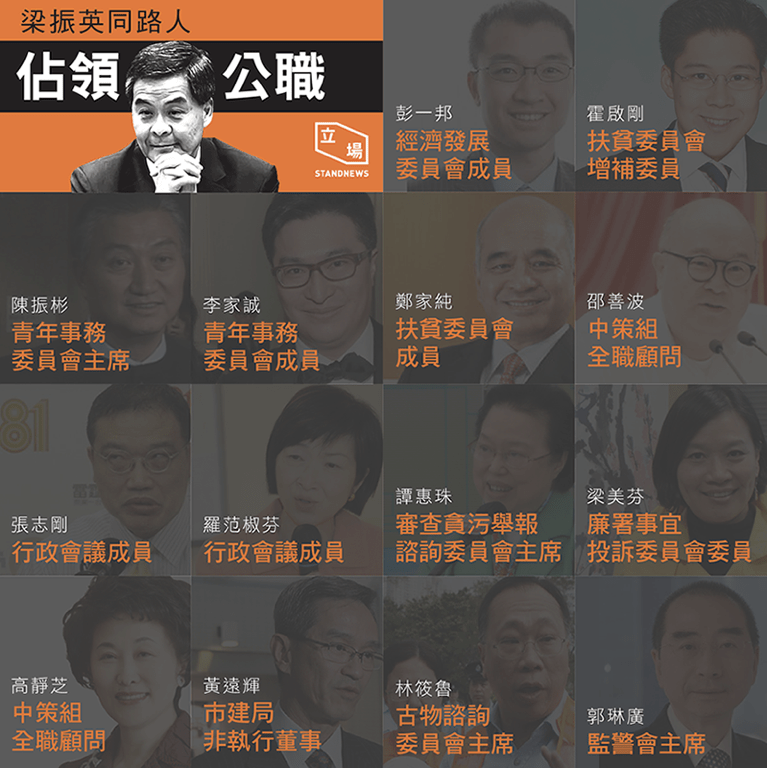
\includegraphics[width=0.7\textwidth]{c20/h-klesson1-032.png}
    \caption{梁振英政府被指嚴重用人唯親} 
\end{figure}

效忠先行的邏輯一層層的推下去,最終做成諮詢政治的失效。港英政府自知其管治沒有選舉授權的基礎,往往會通過各種公眾諮詢活動來收集市民意見,讓大眾感到政府雖然不是由自己選出,但最起碼重要的決定還容許市民一定程度上的參與。同樣的套路在九七後卻明顯失效,雖然各式各樣的諮詢會、聚焦小組、居民會和業界會議越辦越多,許多政策都是政府自以為已經取得大多數人的共識後才提出,結果還是受到排山倒海的反對而要擱置或收回。當中的問題,在於這些諮詢已經變質,成為上述一眾親建制陣營的宣示效忠的場所。近年每當有公眾諮詢,也會有親建制陣營的團體動員支持政府。在市民眼中這些諮詢活動就形同只是為政府製造支持的舞台,自然失去原有籠絡民心的功能。

當公眾開始對各法定組織和公眾諮詢產生懷疑,政府運作便變得舉步維艱。近年最明顯的例子,是醫務委員會改革的爭議。醫委會是香港醫學界自我監管的組織,負責發牌給醫生和處理對他們的投訴。改革的其中一項建議,是引入由病人組織互選的代表,以回應社會對「醫醫相衛」的質疑。然而由於新增代表仍須經行政長官的委任,在香港大學政治干預的陰霾下,輿論擔心將來的行政長官會「有權用盡」,把象徵性的行政長官委任權變成實際介入的權力,借機會讓政府可以把攬過半數的醫委會席位。在公眾對政府的高度不信任之下,本來社會各界都認為有必要進行的醫委會改革,在立法會審議的最後階段被迫擱置。

值的注意的,是就算特區政府想如實執行九七前的一套管治模式,實際難度也大了很多。首先,商界利益本身也在碎片化,政府討好一個利益集團的後果就是換來其他利益集團的圍攻,過去數碼港和西九文化區被指責為地產項目的批評,很大程度上來自那些未能分一杯羹的其他開發商。而隨著社會貧富懸殊越來越嚴重,上流社會越來越被視為脫離大眾,成功拉攏商界利益不見得可以幫助政府介入社會,反而引來官商勾結的指控。選舉政治和公民社會的成熟也使得今天的官民關係和港英時期相去甚遠,民意早已不甘於由這些委員會來代表自己。

與此同時,由於行政長官基本上是由商界利益所選出,而這些利益於投票時主要也是聽命於中央政府,於是特區政府駕馭商界利益的能力也顯得不如港英年代。畢竟,這些商界利益本身各自和中央政府有所聯繫。如是者,過去港英時代政府與商界結盟管治香港的政治經濟結構,在九七之後已經得明顯過時:特區政府既不能團結商界支持其政策,又反過來讓民間覺得政府處處被商界所脅持,過去港英政府在社會中的超然地位固不復見。

另一個變調的認授基礎是公務員系統。當行政長官的權力來源和實踐在制度上有明顯缺陷,由行政長官委任的行政會議成員、政治任命官員以及諮詢和法定組織委員接連出現問題,委任制度以外的公務員系統亦未能幸免。自特區成立以來,香港政府最常見的一個批評,正正是「公務員神話破滅」。在英治時代後期,公務員隊伍往往被讚頌為「高效廉潔」,在東亞地區首屈一指,甚至被譽為公眾利益以及香港制度與核心價值的守衛者。然而特區後,各種施政失誤一浪接一浪,市民對政府的不滿每況愈下,公務員的能力也越來越受到質疑。

香港有超過十六萬名公務員,而政治任命官員只有數十名,真正領導政府日常運作的實為政務職系數百名的政務主任(AO, Administrative Officer)。大學畢業生能成為政務主任的話,會被視為是天之驕子。政務主任一入職的月薪便有約港幣五萬元,另加各類福利津貼,比起一般大學畢業生只得一萬多元的月薪無疑是極為吸引。近年來,每次招考均引來了過萬人應徵,儘管每次招收的名額只有數十人。不過,近年來投考人數的跌幅卻相當明顯,輿論也開始懷疑擔任政務主任是否一份好工作,後面也和公眾對政府的不滿相關。

要理解香港公務員系統面對的挑戰,先要理解公務員守則當中「政治中立」的要求。「政治中立」一詞往往會被認為是大公無私的表現,能夠超越黨派立場來思考,從社會的整體利益出發。但在實際的政府運作當中,「政治中立」的真正意義是要專業地執行上級的任務,不同意可以事前提出,但決定後便一定要服從。只要不違法,必須照做。在英國政黨政治的傳統當中,「政治中立」可確保無講由哪一個政黨上台執政,公務員團隊都會專業和忠實地提供服務。但香港作為中國的一個特區,共產黨在中國的執政地位不容挑戰,「政治中立」便等於把公務員系統變成中共政權在港管治機器的一部分。

在此意義下,市民對公務員團隊的不信任就很容易理解了:即使是以依法執行職務為名的政府行為,也很容易受到質疑。因為在一個非民主制度之下,所謂的「依法」也只是政權自我維護的延伸。在這個制度之下,公務員有三個選擇:一、有政治野心的,可選擇主動配合政權,希望獲得賞識,有日晉身成為問責高官;二、堅持己見的,面對自認為不合理的決定,只有辭職一途,不可拒絕執行;三,利用官僚系統的慣性作消極抵抗。例如上級要求做某件事,下屬可找去一百個要考慮的面向,然後僅僅是走程序便把時間消耗掉,到時候外在政治環境說不定已經改變,使得上級的要求也會因而失效。

說到這兒,問題又回到管治認授的討論。「民無信不立」,香港市民對香港政府的嚴重不信任,已經影響到其日常運作,而這歸根究底出於政府沒有更新管治認授的方法。

拉闊一點來討論,九七前香港人對未來的恐懼,很大程度上建基於八十年代或以前中共在中國大陸引發起的各種政治動盪。與此同時,八十年代的香港正處於快速發展的階段。於是乎,所謂的「五十年不變」,即把當時理解中的中港差異凝固,就被理解為保護香港人生活模式的可接受做法。

來到今天,不難發現這種想法嚴重地與現實脫節。今天的中國已不是八十年代的中國,當時的中國尚在爭取世界各地前來投資,今天的世界反過來擔心中國在海外投資帶來的影響;今天的香港也不再處處講求經濟增長,年輕人更強調的是生活和身分的問題;當時香港的擔憂往往以「社會主義中國」和「資本主義香港」對陣來理解,而中國大陸的經濟改革往往被假設會最終引發政治改革;今天的中國大陸卻由「國退民進」變成「國進民退」,並實行一套無遠弗屆的國家資本主義,而中產階層由於成為既得利益者,由下而上的政治改革仍屬空談。換言之,九七前港英管治所處的時空背景,和今天的已經差天共地。

不少公共行政的學者都不約而同地指出,戰後香港的管治制度雖然不民主,但在中國威脅面前會做到自我克制,主動消除濫權,致力為華人社會提供良好管治。換句話說,九七前的善治並非純粹英國出於菩薩心場贈予香港,而有地緣政治的考量在其中。來到九七之後,中英二元權力結構不再存在,公眾對管治認授的訴求卻有增無減,管治制度理應從集權者的自我約束轉變為民主制度的互相制衡,才能面對新時代的需要。當這改變沒有發生,管治就出現各種斷裂。

九七前的政治和社會環境使得港英政府能面對其管治認授的挑戰,把同一套系統放到今天,無論是香港所處的政治環境或是香港社會本身都已變得大不一樣,同一套的制度在今天失效十分合理。如是者,「五十年不變」便從一個保證變成了一種咀咒,阻延香港本來應該面對的改變。以為接收了英國人留下來的殖民管治框架,換個頭目據為己用,便可以順利管治香港社會,是個相當錯誤的想法。要解決香港今天的管治問題,不能再走過去殖民地的舊路,而該直視一國兩制運行二十年來所揭示的制度性問題。



伸延閱讀:

曾銳生(2007):《管治香港:政務官與良好管治的建立》,香港:香港大學出版社。

李彭廣(2012):《管治香港:解英國解密檔案的啟示》,香港:牛津大學出版社。

Scott I (2003) The Disarticulation of Hong Kong’s Post-Handover Political System, in Sing M (ed) \textit{Hong Kong Government and Politics}. p. 663-694

Fong B (2015) \textit{Hong Kong’s Governance Under Chinese Sovereignty: The Failure of the State-Business Alliance after 1997}. Routledge: London and New York.

網上資源:

\href{https://thestandnews.com/politics/梁振英同路人-佔領公職/ }{立場報道(2015):〈梁振英同路人 佔領公職〉:立場新聞,2015年1月16日}